\chapter{Thiết kế cơ sở dữ liệu}

\section{Mô hình dữ liệu tổng quan}
Mô hình dữ liệu được tổ chức thành các nhóm Identity, Farm, Sensor, UAV, Mission và Alert.
\begin{table}[H]
\centering
\caption{Phân nhóm bảng}
\begin{tabularx}{\textwidth}{p{3cm}X}
\toprule
Nhóm & Bảng\\
\midrule
Identity & ROLE, USER\\
Farm & FARM, ZONE\\
Sensor & SENSOR\_TYPE, SENSOR\_NODE, SENSOR\_DATA, THRESHOLD\\
UAV & UAV, MOBILE\_GATEWAY\\
Mission & MISSION, MISSION\_SENSOR, WAYPOINT, MISSION\_COLLECTION, MISSION\_NOTE\\
Alert & ALERT, NOTIFICATION, ALERT\_HANDLING\\
\bottomrule
\end{tabularx}
\end{table}

\section{ERD tổng quan}
\begin{figure}[H]\centering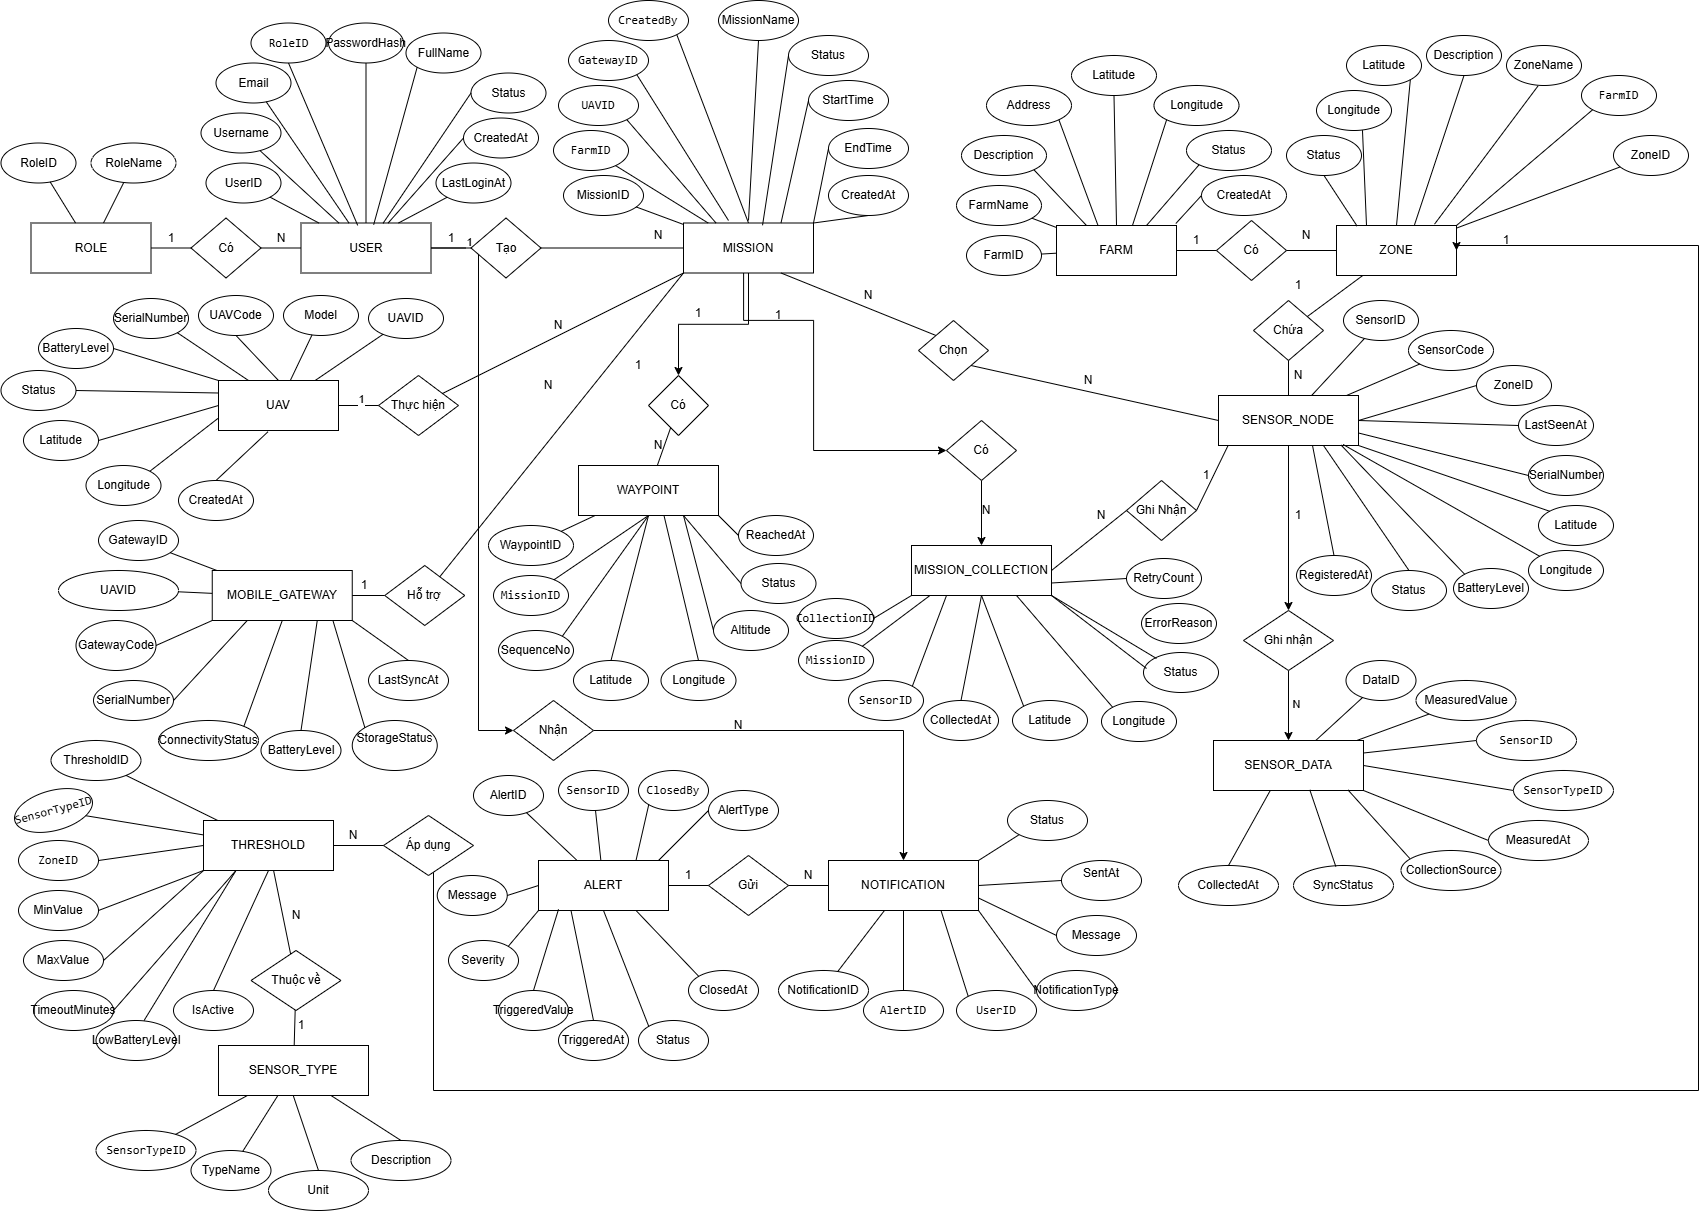
\includegraphics[width=0.98\textwidth,height=0.68\textheight,keepaspectratio]{figures/erd2.png}\caption{Mô hình ERD tổng quan}\end{figure}

\section{Danh mục bảng}
\begin{longtable}{p{4cm}p{10cm}}
\caption{Danh mục bảng và mục đích}\label{tab:tables}\\
\toprule
Bảng & Mục đích\\
\midrule
\endfirsthead
\toprule
Bảng & Mục đích\\
\midrule
\endhead
1.USER & Tài khoản, thông tin đăng nhập của người dùng.\\
2.ROLE & Vai trò của người dùng.\\
3.FARM & Thông tin nông trại.\\
4.ZONE & Khu vực thuộc Farm.\\
5.SENSOR\_NODE & Thiết bị cảm biến được đăng ký tại zone.\\
6.SENSOR\_TYPE & Loại chỉ số cảm biến và đơn vị đo.\\
7.SENSOR\_\\MEASUREMENT & là kết quả mà thiết bị đó đo được tại một thời điểm cụ thể theo Sensor Node.\\
8.UAV & Thiết bị bay được quản lý trong hệ thống.\\
9.UAV\_GATEWAY & Gateway gắn với UAV, phục vụ collection/sync.\\
10.TELEMETRY\_DATA & Lưu các thông tin trạng thái và hoạt động của UAV trong quá trình thực hiện một mission\\
11.COLLECTION\_\\MISSION& Nhật ký từng lần thu thập, retry và lỗi.\\
12.MISSION\_\\SENSOR & Bảng liên kết mission--sensor.\\
13.WAY\_POINT & Các điểm tuyến của mission.\\
14.OFFLINE\_DATA\_\\RECORD & lưu tạm dữ liệu mà UAV Gateway đã thu thập được khi chưa thể kết nối với Server.\\
15.SYNCLOG & ghi nhận và theo dõi quá trình đồng bộ dữ liệu từ UAV Gateway lên hệ thống trung tâm.\\
16.THRESHOLD & điều kiện để phát hiện bất thường.\\
17.ALERT & Cảnh báo phát sinh từ sensor data.\\
18.NOTIFICATION & Thông báo gửi cho user.\\
19.REPORT & Báo cáo.\\
20.DEVICE\_\\CREDENTIAL & Bảo mật thiết bị.\\
\bottomrule
\end{longtable}

\section{Quan hệ chính}
\begin{table}[H]
\centering
\caption{Các quan hệ chính}
\begin{tabularx}{\textwidth}{p{5cm}p{3cm}X}
\toprule
Cha & Cardinality & Con\\
\midrule
1.ROLE & 1:N & USER\\
2.FARM & 1:N & ZONE\\
3.ZONE & 1:N & SENSOR\_NODE\\
4.SENSOR\_NODE & 1:N & SENSOR\_MEASUREMENT\\
5.SENSOR\_TYPE & 1:N & SENSOR\_MEASUREMENT\\
6.FARM & 1:N & COLLECTION\_MISSION\\
7.UAV & 1:N & COLLECTION\_MISSION\\
8.UAV\_GATEWAY & 1:N & COLLECTION\_MISSION\\
9.USER & 1:N & COLLECTION\_MISSION\\
10.COLLECTION\_\\MISSION & N:N & SENSOR\_NODE\\
11.COLLECTION\_\\MISSION & 1:N & WAY\_POINT\\
12.UAV & 1:N & TELEMETRY\_DATA\\
13.COLLECTION\_\\MISSION & 1:N & TELEMETRY\_DATA\\
14.SENSOR\_TYPE & 1:N & THRESHOLD\\
15.ZONE & 1:N & THRESHOLD\\
16.SENSOR\_NODE & 1:N & ALERT\\
17.SENSOR\_\\MEASUREMENT & 1:N & ALERT\\
18.THRESHOLD & 1:N & ALERT\\
19.ALERT & 1:N & NOTIFICATION\\
20.USER & 1:N & NOTIFICATION\\
21.UAV\_GATEWAY & 1:N & OFFLINE\_DATA\_RECORD\\
22.SENSOR\_NOTE & 1:N & OFFLINE\_DATA\_RECORD\\
23.UAV\_GATEWAY & 1:N & SYNCLOG\\
24.USER & 1:N & REPORT\\
25.COLLECTION\_\\MISSION & 1:N & MISSION\_SENSOR\\
26.SENSOR\_NODE & 1:N & MISSION\_SENSOR\\
\bottomrule
\end{tabularx}
\end{table}

\section{Khóa chính, khóa ngoại và chuẩn hóa}
Mỗi entity chính có khóa chính định danh. Quan hệ 1:N dùng foreign key ở phía N. Quan hệ N:M giữa MISSION và SENSOR\_NODE dùng MISSION\_SENSOR với khóa ghép (MissionID, SensorID). Việc tách FARM, ZONE, SENSOR\_NODE, SENSOR\_TYPE và SENSOR\_DATA giúp giảm lặp dữ liệu. THRESHOLD được tách khỏi lịch sử measurement để thay đổi cấu hình mà không phải sửa dữ liệu lịch sử.

Các constraint nên gồm PRIMARY KEY, FOREIGN KEY, UNIQUE cho mã nghiệp vụ khi phù hợp, NOT NULL cho cột bắt buộc và CHECK cho các miền giá trị như battery level và MinValue $\le$ MaxValue.

\section{Index đề xuất}
\begin{itemize}
\item SENSOR\_DATA(SensorID, MeasuredAt).
\item SENSOR\_DATA(SensorTypeID, MeasuredAt).
\item MISSION\_COLLECTION(MissionID, Status).
\item ALERT(SensorID, Status, TriggeredAt).
\item NOTIFICATION(UserID, Status, SentAt).
\item WAYPOINT(MissionID, SequenceNo).
\end{itemize}

\section{Schema chi tiết}
\begin{figure}[H]\centering
\includegraphics[width=0.92\textwidth,height=0.62\textheight,keepaspectratio]{figures/schema_user_farm_zone.png}\caption{Schema nhóm User, Farm và Zone}\end{figure}
\begin{figure}[H]\centering
\includegraphics[width=0.92\textwidth,height=0.62\textheight,keepaspectratio]{figures/schema_sensor_threshold.png}\caption{Schema nhóm Sensor và Threshold}\end{figure}
\begin{figure}[H]\centering
\includegraphics[width=0.92\textwidth,height=0.62\textheight,keepaspectratio]{figures/schema_uav_mission.png}\caption{Schema nhóm UAV, Gateway và Mission}\end{figure}
\begin{figure}[H]\centering
\includegraphics[width=0.92\textwidth,height=0.62\textheight,keepaspectratio]{figures/schema_collection_alert.png}\caption{Schema nhóm Collection và Alert}\end{figure}
